% !TEX root = master.tex
\chapter{Evaluation der Ergebnisse}
\label{chapter:4}
\section{Ergebnisse}
\begin{table}[h]
	\centering
	\begin{tabularx}{\textwidth}{|c|X|c|}
		\hline
		\multirow{34}{*}[4ex]{\rotatebox[origin=c]{90}{\centering \textbf{Visualisierung}}} & \textbf{Anforderungen} & \textbf{Erfüllt} \\
		\cline{2-3}
		& Das Video wurde durch Python und Manim animiert und gerendert & $\square$ \\[4ex]
		& Die Länge des Videos überschreitet nicht 15 Minuten & $\square$ \\[4ex]
		& Das Video ist vollständig vertont & $\square$ \\[4ex]
		\cline{2-3}
		\multirow{44}{*}[10ex]{\rotatebox[origin=c]{90}{\centering \textbf{Implementierung}}} & Das Konzept von NEAT soll vollständig und verständlich sein & $\square$ \\[4ex]
		& Visualisierungsgrundlagen sollen berücksichtigt werden & $\square$ \\[4ex]
		& Ein roter Faden sollte erkennbar sein & $\square$ \\[4ex]
		& Das Video soll ansprechend animiert sein & $\square$ \\[4ex]
		\hline
		& NEAT Algorithmus implementieren und testen & $\square$ \\[4ex]
		& Lander durch NEAT Algorithmus steuern & $\square$ \\[4ex]
		& Aktionen aus 8-dimensionalen Input Vektoren ableiten & $\square$ \\[4ex]
		& Agent soll mindestens 200  Punkte erreichen & $\square$ \\[4ex]
		\cline{2-3}
		& Programm soll replizierbar sein & $\square$ \\[4ex]
		\hline
	\end{tabularx}
	\caption{Checkliste für funktionale und nicht funktionale Anforderungen}
\end{table}

Um das Projekt sachgemäß zu evaluieren, wird im Folgenden die Liste der Anforderungen auf ihre Erfüllung hin überprüft.

Die Bewertung der Visualisierung basiert auf dem eingereichten Video. Aus diesem lässt sich erkennen, dass das gesamte Video im Manim-Stil erstellt wurde. Der zugehörige Quellcode ist in einem GitHub-Repository dokumentiert \cite{githubdoc}. Die Länge des Videos bleibt unter 15 Minuten, und es ist vollständig vertont. Basierend auf dem Feedback von Kommilitonen wurde das Konzept von NEAT verständlich vermittelt. Dabei hat der Ersteller des Videos aktiv auf wichtige Visualisierungsgrundlagen, wie Farbkomposition und Lesbarkeit, geachtet. Die durchgängige Struktur und Verständlichkeit wird durch das zuvor angefertigte Storyboard sichergestellt. Das Video wurde als angenehm anzusehen bewertet, was größtenteils auf die Qualität der Animationen zurückzuführen ist.

\begin{figure}[h] % 'h' bedeutet, dass LaTeX versuchen wird, das Bild an dieser Stelle einzufügen
	\centering % Zentriert das Bild horizontal
	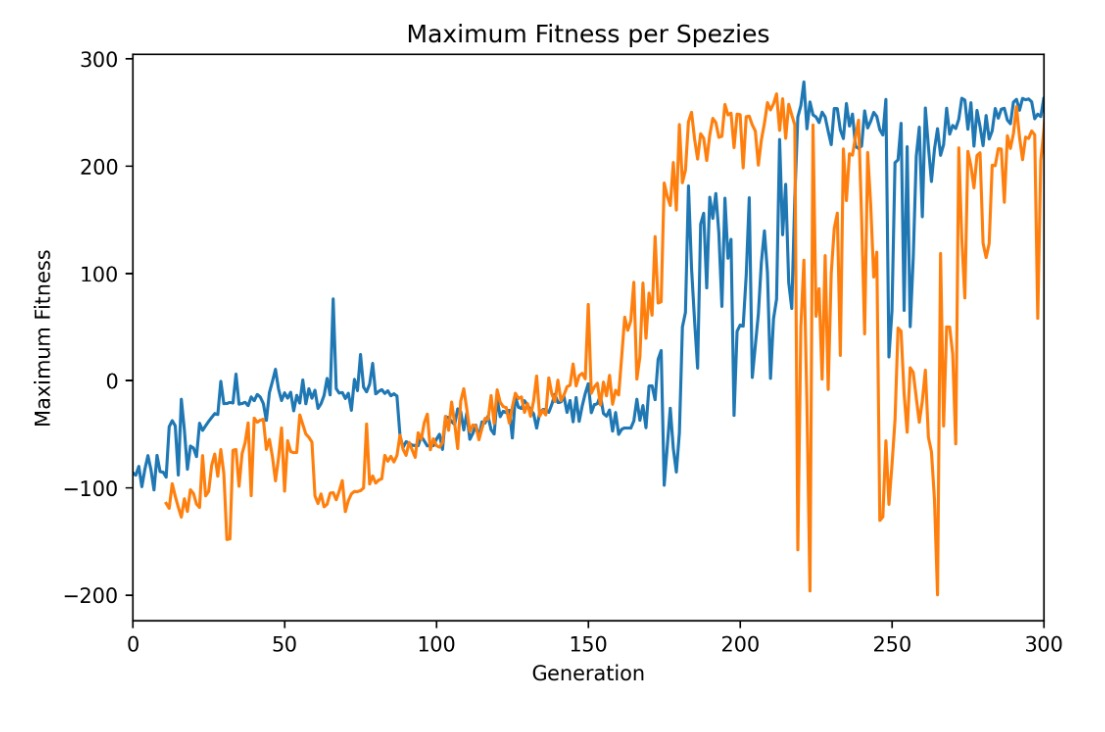
\includegraphics[width=1\textwidth]{\imagedir/species.jpg} % Ersetzen Sie 'meinbild.png' durch den Dateinamen Ihres Bildes
	\caption{Abbildung des Fitnessverlaufs der beiden besten Spezien} % Fügen Sie Ihre Bildbeschriftung hier ein
\end{figure}

Die Evaluierung der Implementierung basiert, wie aus der Grafik ersichtlich, auf der maximalen Fitness, die von einer Spezies erreicht wurde. Eine Spezies, die eine Fitness von 200 erreicht, gilt dabei als Lösung. Die Fitness beruht auf einer Metrik, die eine Kombination aus Geschwindigkeit, Triebwerksauslastung, Rotation und Nähe zum Ziel darstellt \cite{gymnasiumdoc}. Die dargestellten Grafiken zeigen die beiden besten Spezies mit ihren entsprechenden Fitness-Leveln über mehrere Generationen hinweg. Es ist erkennbar, dass der Score von 200 überschritten wird, jedoch eine hohe Fluktuation in der Leistung besteht. Dies könnte auf das Konzept der Spezies zurückzuführen sein, die auch nicht optimale Netzwerke beinhalten können. Das Gesamtergebnis wurde ausschließlich durch NEAT-basiertes Lernen auf den Input-Vektoren erzielt, welches von Grund auf in einer strukturierten Form in Python implementiert wurde. Verschiedene Spezies haben zur Zielerreichung unterschiedliche Strategien angewandt. Der Entwicklungsprozess reichte von zufälliger Steuerung über eine \enquote{Kopf-zuerst}-Strategie bis hin zur finalen Version, die sich zuerst fallen lässt und dann relativ spät die Triebwerke zur Abfederung aktiviert und ins Ziel fliegt. Es wurde ebenfalls festgestellt, dass die kontinuierliche Aktivierung der Triebwerke bessere Ergebnisse erbrachte als die absolute Aktivierung. Während die Anfangsversion das Ziel nie erreichte, konnte die finale Spezies durch NEAT-basiertes Lernen und Selektion die Rakete jedes Mal landen.

\begin{table}[h]
	\centering
	\begin{tabularx}{\textwidth}{|c|X|c|}
		\hline
		\multirow{34}{*}[4ex]{\rotatebox[origin=c]{90}{\centering \textbf{Visualisierung}}} & \textbf{Anforderungen} & \textbf{Erfüllt} \\
		\cline{2-3}
		& Das Video wurde durch Python und Manim animiert und gerendert & $\checkmark$ \\[4ex]
		& Die Länge des Videos überschreitet nicht 15 Minuten & $\checkmark$ \\[4ex]
		& Das Video ist vollständig vertont & $\checkmark$ \\[4ex]
		\cline{2-3}
		\multirow{44}{*}[10ex]{\rotatebox[origin=c]{90}{\centering \textbf{Implementierung}}} & Das Konzept von NEAT soll vollständig und verständlich sein & $\checkmark$ \\[4ex]
		& Visualisierungsgrundlagen sollen berücksichtigt werden & $\checkmark$ \\[4ex]
		& Ein roter Faden sollte erkennbar sein & $\checkmark$ \\[4ex]
		& Das Video soll ansprechend animiert sein & $\checkmark$ \\[4ex]
		\hline
		& NEAT Algorithmus implementieren und testen & $\checkmark$ \\[4ex]
		& Lander durch NEAT Algorithmus steuern & $\checkmark$ \\[4ex]
		& Aktionen aus 8-dimensionalen Input Vektoren ableiten & $\checkmark$ \\[4ex]
		& Agent soll mindestens 200 Punkte erreichen & $\checkmark$ \\[4ex]
		\cline{2-3}
		& Programm soll einfach und replizierbar sein & $\checkmark$ \\[4ex]
		\hline
	\end{tabularx}
	\caption{Erfüllte Checkliste für funktionale und nicht funktionale Anforderungen}
\end{table}

Basierend auf diesen Ergebnissen kann die Evaluation als komplett angesehen werden. Alle festgelegten technischen und nicht-technischen Anforderungen konnten umgesetzt werden, sodass das Projekt vollständig nach den Vorgaben implementiert wurde.

\section{Handlungsempfehlungen}
In diesem Beispiel konnte NEAT sehr gute Ergebnisse erzielen und die Anforderungen des Spiels meistern. Der Algorithmus fand eine sehr gute Lösung und konnte die Eingabewerte entsprechend generalisieren und verwenden. Vermutlich hätte ein Deep Learning- oder Reinforcement Learning-Ansatz dies ebenso geschafft, allerdings mit einer wesentlich einfacheren und generalistischeren Implementierung. Daher stellt sich die Frage nach der Zukunft der genetischen Algorithmen. Es scheint, dass NEAT für bestimmte Zwecke sehr gut funktioniert, jedoch eine relativ strikte Struktur voraussetzt. Ein weiteres Problem ist die hohe Fitness-Volatilität zwischen den Epochen, die das Lernen in späteren Phasen verlangsamen kann. Für einen allgemeineren Ansatz hat sich nach unserer Einschätzung Deep Learning als Favorit herauskristallisiert, da es einen generalistischen Ansatz für Lernprobleme verfolgt. In diesem Bereich gibt es zudem erhebliches Forschungspotential, das noch ausgeschöpft werden kann. Eine Kombination von auf natürlichen Prinzipien basierender Selektion während des Deep Learning-Prozesses ist allerdings eine denkbare Möglichkeit.